%% CCF-A conference paper (ACM sigconf format; KDD/CIKM/WWW/SIGIR-ready).
%% Compile:  pdflatex main ; bibtex main ; pdflatex main ; pdflatex main
%% Requires acmart.cls (TeX Live / Overleaf). Figures in sections/figures/.
\documentclass[sigconf,nonacm]{acmart}

\usepackage{booktabs}
\usepackage{amsmath,amssymb}
\usepackage{graphicx}
\usepackage{xcolor}
\graphicspath{{sections/figures/}}

\settopmatter{printacmref=false}
\renewcommand\footnotetextcopyrightpermission[1]{}
\pagestyle{plain}

\newcommand{\rk}[1]{\textsf{#1}}
\newcommand{\mt}[1]{\texttt{#1}}

\begin{document}

\title{Detection Is Not Edge: A Leakage-Free, Cost-Aware Audit of LLM Agents,
Regime Models, and Candlestick Motifs for Stock-Movement Onset on Chinese A-Shares}

\author{Xingke Gao}
\affiliation{%
  \institution{Independent Quantitative Research (V12.31 production system)}
  \city{}\country{China}}
\email{fanatxmu@gmail.com}

\renewcommand{\shortauthors}{Gao}

\begin{abstract}
We report a deployment-realistic audit of machine-learning and large-language-model
(LLM) methods for \emph{movement-onset detection} --- predicting the \emph{start} of
a price move --- on the Chinese A-share market, anchored to a deployed production
system (V12.31; documented $\alpha$ $+2.236$pp/month, Sharpe $2.20$). We package the
production logic as \textbf{V12-Agentic}, a four-agent framework (Macro Regime
Monitor, Alpha Factor Explorer, Pattern Core, Backtest \& Verifier), and a
knowledge-encoding methodology that converts tacit operator expertise into a
structured agent prompt. Against this framework we run a rigorous, mostly negative
evaluation on a 5.27M-anchor panel under a strict leakage-free walk-forward,
realistic A-share transaction costs, date-clustered bootstrap confidence intervals
(CIs), and the Deflated Sharpe Ratio (DSR). Six findings follow. (\textbf{C1--C2})
the knowledge-encoding procedure and the agentic framework; (\textbf{C3}) apparent
hybrid-over-LGBM gains are \emph{within date-clustered noise}; (\textbf{C4}) a
quarter-conditional oracle bounds any router at $+0.39$pp Top-10\%; (\textbf{C5}) on
a leakage-free substrate the \emph{identified} LLM contribution to onset is
$\approx 0$ (raw $+0.033$, expert $+0.006$; both span zero), LLM-as-weak-supervisor
is harmful ($-0.149$), and a cross-market de-biasing estimator collapses public
benchmark ``skill'' (67--80\%) to chance; (\textbf{C6}) candlestick onset
information is real, regime-conditional, cross-period-stable, and even directionally
monotone, yet its gross edge ($\approx 0.1\%/$5d) is \emph{below the transaction-cost
floor} --- information, not tradable alpha. Reimplementing three 2025--26 SOTA
baselines (regime LightGBM, two-level abstention, NMI information theory) under our
protocol, \emph{none survives}. We connect these nulls to two architectural limits
of LLMs --- proactive interference and mode collapse. Across 11 research lines and
60+ method/arm comparisons, no configuration yields deployable alpha from public
features; the contribution is the honest evaluation machinery and a precise
localization of \emph{why} detection $\neq$ edge.
\end{abstract}

\keywords{stock movement prediction, movement onset, LLM agents, data leakage,
transaction costs, mutual information, regime models, honest evaluation, A-shares}

\maketitle

%======================================================================
\section{Introduction}\label{sec:intro}

Stock-movement prediction has been studied for decades, yet a persistent gap
separates academic methods from deployed systems. Academic work typically evaluates
on stratified subsets that overrepresent the event of interest (e.g.\ 25\% positive
class), while deployment must operate under the true marginal ($<$10\%). Recent LLM
agents~\cite{yu2024finagent,hu2024alphaforge,li2024tradinggpt} intensify the gap:
whether they add genuine alpha in a production pipeline, and how to combine them with
mature tabular models, is poorly studied at scale. The cost of producing a
beautiful-but-worthless backtest with AI assistance is now near zero, which
accelerates over-fitting and false discovery rather than solving research.

We address this with \textbf{V12-Agentic}, a four-agent framework grounded in a
deployed A-share system (V12.31), and subject it to a deliberately adversarial,
leakage-free, cost-aware evaluation. The A-share setting is an ideal testbed:
(i) most retail-accessible stocks \emph{cannot be shorted}, so a bearish signal is an
avoidance criterion, not a tradeable direction; (ii) onset events are sparse
($\approx 8\%$); (iii) recurring ``disaster months'' induce regime non-stationarity.

\paragraph{Contributions.} This paper makes six contributions. The methodological
novelty is C1, C2, and the leakage-free \emph{identification} framework C5; C3--C4
and C6 are honest, deployment-realistic empirical findings rather than new techniques.

\begin{itemize}
\item \textbf{C1 --- Knowledge encoding.} A procedure converting tacit production
knowledge (onset rules, disaster signals, asymmetric short-sale constraints) into a
$\sim$5{,}500-character structured agent prompt (\S\ref{sec:arch}, App.~A).
\item \textbf{C2 --- V12-Agentic architecture.} A four-agent decomposition mapping to
a real production codebase (\S\ref{sec:arch}).
\item \textbf{C3 --- Hybrid effects are within noise.} A stratified ``+54\% over
LGBM'' reverses to $-15\%$ on a random sample; three controlled experiments show this
is \emph{not} a base-rate mechanism but date-clustered noise: the headline gap is
$+0.72$pp, 95\% CI $[-0.56,+2.05]$pp (\S\ref{sec:noise}).
\item \textbf{C4 --- Quarter-conditional headroom.} An oracle upper bound of
$+0.39$pp Top-10\% for any online regime router; our routers capture $\approx 0$ of it
(\S\ref{sec:oracle}).
\item \textbf{C5 --- Leakage-free identification.} Treating leakage-freeness as an
identification condition, the LLM's incremental contribution to A-share onset is
$\approx 0$; weak supervision is harmful; a de-biasing estimator collapses
contaminated-benchmark skill to chance (\S\ref{sec:identify}).
\item \textbf{C6 --- Detection is not edge.} Candlestick onset information is real,
regime-conditional, cross-period-stable, and directionally monotone, yet sub-cost
(\S\ref{sec:motif}); reimplemented SOTA regime/abstention/information-theory
baselines are \emph{also} sub-cost under our protocol (\S\ref{sec:bench}).
\end{itemize}

Figure~\ref{fig:tree} previews all 11 lines and 60+ methods compared.

\begin{figure*}[t]
\centering
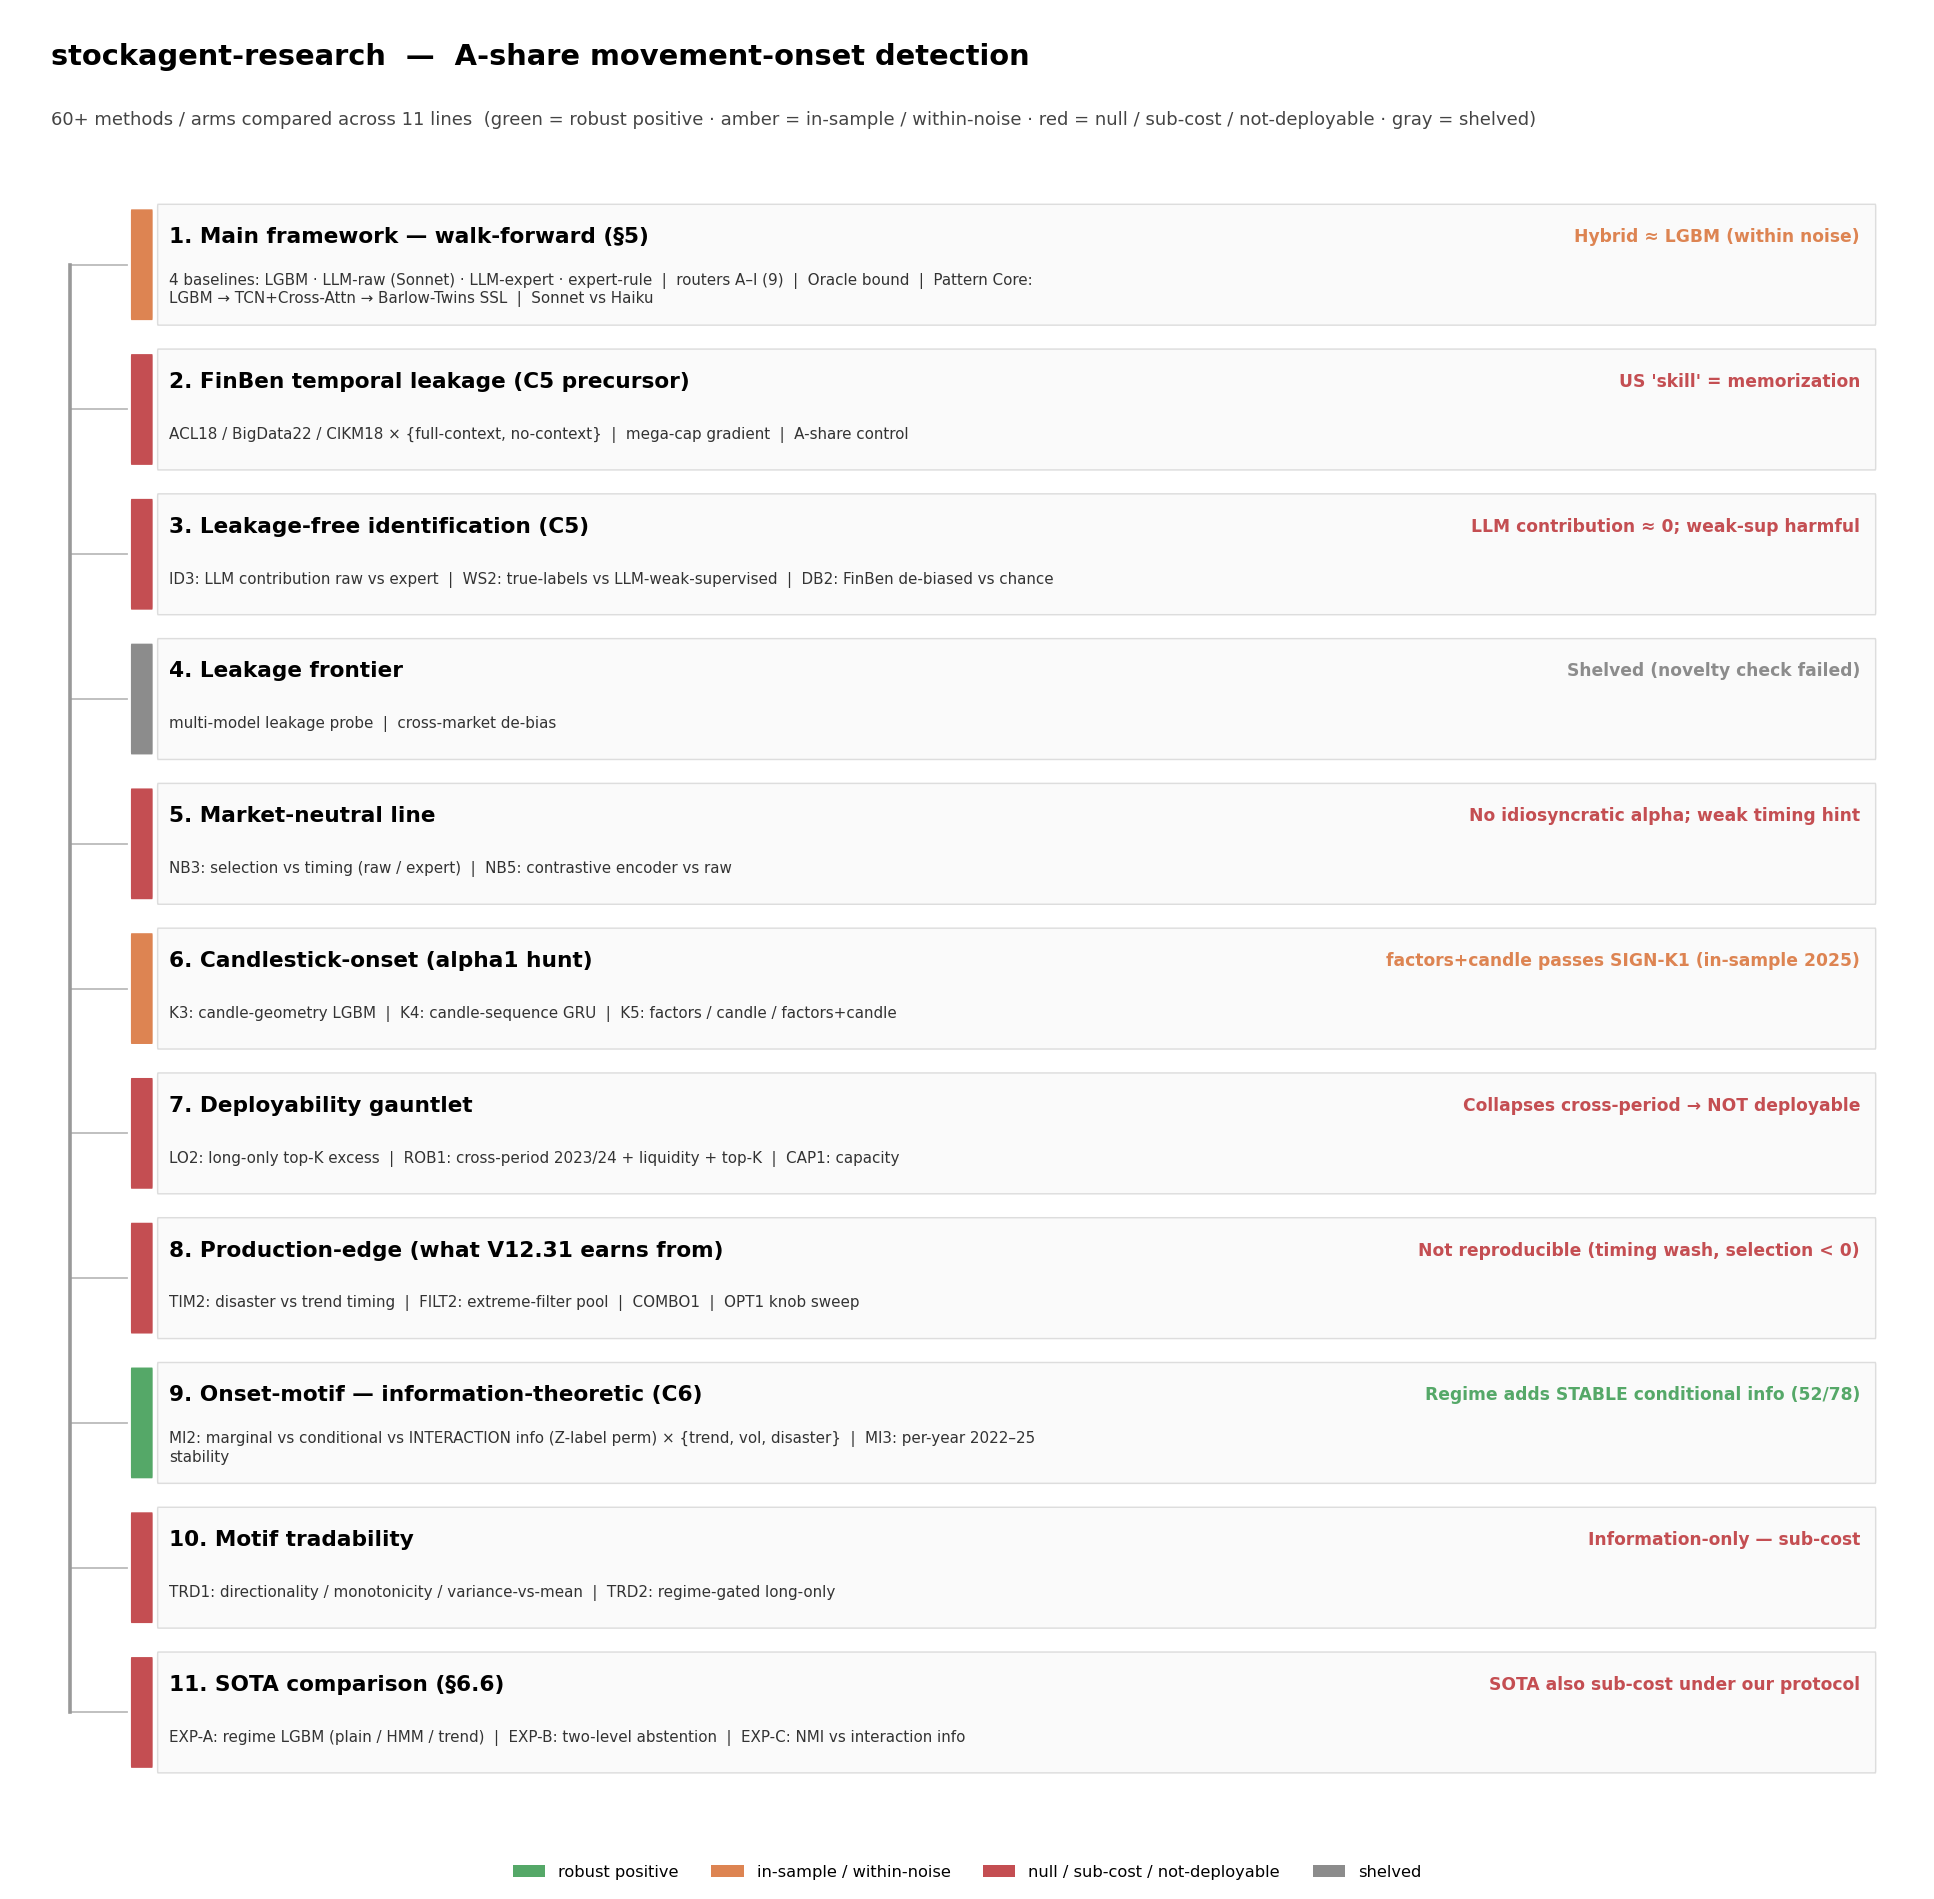
\includegraphics[width=\textwidth]{methods_tree.png}
\caption{Overview of every method/arm compared across the project's 11 research
lines, colour-coded by verdict (green: robust positive; amber: in-sample /
within-noise; red: null / sub-cost / not deployable; gray: shelved). Across 60+
comparisons, only the onset-motif \emph{information} (C6) is a robust positive, and
it is sub-cost.}
\label{fig:tree}
\end{figure*}

%======================================================================
\section{Related Work}\label{sec:related}

\paragraph{Stock movement prediction.} Triple-barrier labeling~\cite{lopezdeprado2018advances},
graph and attention models (HIST~\cite{xu2021hist}, MASTER~\cite{li2024master},
StockMixer~\cite{fan2024stockmixer}, FactorVAE~\cite{duan2022factorvae}), and gradient
boosting~\cite{ke2017lightgbm,friedman2001greedy} are standard. Recent work questions
optimal supervision horizons (Label Horizon Paradox) and the practicality of chart-based
deep learning, the latter concluding that DNN chart predictors create false positives
once temporal context is respected --- an independent echo of our C5/C6.

\paragraph{LLM agents in finance.} FinAgent~\cite{yu2024finagent},
AlphaForge~\cite{hu2024alphaforge}, FinRobot~\cite{wang2024finrobot},
TradingGPT~\cite{li2024tradinggpt} and domain-tuned LLMs evaluate mostly on curated
benchmarks. A growing line documents temporal leakage and ``profit mirages'' in
LLM-finance~\cite{glasserman2023lookahead,sarkar2024lookahead,lopezlira2023chatgpt,profitmirage2025,ktdfin2026}.

\paragraph{Architectural limits of LLMs as alpha generators.} Two recent results give
a mechanistic basis for \emph{why} our identified LLM contribution is null rather than
merely small. \emph{Proactive interference}~\cite{wang2025proactive} shows LLM retrieval
of the latest value in a stream of related updates decays log-linearly toward zero as
prior updates accumulate --- a working-memory bottleneck independent of context-window
size and not fixed by prompting, across 30+ models. This undercuts feeding long
multi-period histories to an LLM and expecting it to track the \emph{current} state.
\emph{Mode collapse}~\cite{jiang2025hivemind} (NeurIPS 2025 Best Paper) documents an
``Artificial Hivemind'' across 70+ models: open-ended generations converge both within a
model and across families, so neither temperature nor ensembling restores diversity.
Because alpha lives in the long tail, a mode-seeking generator structurally reproduces
already-arbitraged ``traditional wisdom.'' These limits frame C5 and C6 as expected
consequences of using an LLM as ideator/predictor rather than as a rigorous
execution-and-falsification engine under human-supplied hypotheses.

\paragraph{Information theory, transaction costs, multiple testing.} We use interaction
information~\cite{mcgill1954} and conditional mutual information~\cite{coverthomas2006}
with permutation inference~\cite{ojala2010permutation}; the anomaly-cost-erosion
literature~\cite{novymarx2016taxonomy} and regime-conditional returns~\cite{cooper2004market}
contextualize C6; and we report the Deflated Sharpe Ratio~\cite{bailey2014deflated} to
correct for the many strategy variants tried.

%======================================================================
\section{Movement Onset: Problem and Asymmetry}\label{sec:problem}

For $(i,t)$ with adjusted close $P_{i,t}$, let $r^{(h)}_{i,t}=P_{i,t+h}/P_{i,t}-1$.

\noindent\textbf{Definition 1 (Bullish onset).} A bullish onset occurs at $(i,t)$ iff
(1) forward magnitude $r^{(H)}_{i,t}\ge\Delta^+$; (2) bounded drawdown
$\min_{0\le h\le H}P_{i,t+h}/P_{i,t}\ge 1-\Delta^-$; (3) backward context
$\sum_{s=t-W}^{t-1}\log(P_{i,s+1}/P_{i,s})\le\tau$. In V12.31,
$(H,\Delta^+,\Delta^-,W,\tau)=(5,0.10,0.05,5,0.08)$. Condition (3) prevents labeling
already-trending stocks as onsets.

\paragraph{Asymmetric short-sale constraint.} Most A-shares cannot be shorted, so a
bearish onset can only \emph{remove} a stock from a long-only pool (Bearish-as-Filter),
and negative peer information carries disproportionate predictive
weight~\cite{cooper2004market}. This motivates a two-track design: a long-bullish track
plus a bearish-onset filter.

\paragraph{Sparse events and sampling.} The bullish onset rate is $\approx 8.0\%$.
Three regimes appear: stratified-PoC (25\% positive), walk-forward-random (7.9--9.4\%,
the deployment distribution), and quarter-stratified. We show that stratified-PoC
overstates hybrid advantage (\S\ref{sec:noise}).

\paragraph{Evaluation targets.} RankIC (per-date cross-sectional Spearman vs
$r^{(5)}$), Top-$K$ return and winrate ($K\in\{10\%,20\%\}$), with 1000-resample
date-clustered bootstrap CIs. For tradability we additionally report long-only top-$K$
market-excess net of realistic A-share round-trip cost, annualized Sharpe, and DSR.

%======================================================================
\section{V12-Agentic Architecture}\label{sec:arch}

Four agents operate in a producer--consumer cascade.

\paragraph{Macro Regime Monitor.} A daily binary disaster flag
$z^M_t=\mathbb{1}[(A_t+B_t+C_t)\ge 2]$ from index-AND ($A$), volume-OR ($B$), and
sector inner-vote ($C$) signals. On D1 it flags 12/1062 days (1.13\%).

\paragraph{Alpha Factor Explorer.} Maintains 153 technical/fundamental factors plus 8
concept-heat factors; ten forward-looking columns (\mt{r5}--\mt{r40},
\mt{dd5}--\mt{dd40}; $\mathrm{spearman}(\mt{r5},r^{(5)})=0.898$) are blacklisted,
leaving 165 effective features. Its core asset is the \textbf{expert-knowledge prompt}
(C1): a four-round interview elicitation encoding the bullish-onset rules
($C1$ bottoms-rising, $C2$ above-5d-low, $C3$ MA pattern, $C4$ volume), the bearish
asymmetry, and the disaster composite. The executable rule fires at 7.76\%, matching
the 8\% production label.

\paragraph{Pattern Core.} Emits per-stock onset probabilities. \emph{Phase 1} is
LightGBM (63 leaves, 500 rounds, leakage-protected). \emph{Phase 2} is a TCN-causal
encoder (dilations $\{1,2,4,8\}$, $d{=}64$) with bidirectional spatio-temporal
cross-attention (4 heads; 119{,}171 params). \emph{Phase 3} pretrains that encoder with
Barlow Twins~\cite{zbontar2021barlow} SSL on unlabeled anchors then finetunes with differential learning
rates. Table~\ref{tab:pattern} compares phases.

\paragraph{Backtest \& Verifier.} Combines Pattern Core and LLM signals via nine
routing strategies (A--I: confidence, stratum, soft-ensemble, avoid-expert,
LGBM-floor-LLM-boost, disaster-aware, disagreement-boost, regime-ensemble,
onset-aware), then runs walk-forward evaluation with bootstrap CIs.

\begin{table}[t]
\centering\small
\caption{Pattern Core phases (mean over 3 walk-forward splits). Phase 3 matches
Phase 1 with $116\times$ less labeled data and no deployment-time LLM cost.}
\label{tab:pattern}
\begin{tabular}{lccc}
\toprule
Phase & Labeled data & RankIC & Top-10\% \\
\midrule
Phase 1: LGBM & 3.5M anchors & $+0.088$ & $+1.63\%$ \\
Phase 2: TCN & 100K ($35\times$ less) & $+0.060$ & $+1.61\%$ \\
Phase 3: BT-SSL+TCN & 30K lab.\ + 100K unlab. & $+0.077$ & $+1.63\%$ \\
\bottomrule
\end{tabular}
\end{table}

%======================================================================
\section{Experiments}\label{sec:exp}

\paragraph{Dataset.} \textbf{D1} (Tushare Pro, A-shares 2022-01-04 to 2026-05-27):
5{,}275{,}812 anchors, 5{,}434 stocks, 1{,}062 trading days, 185 columns; onset rate
8.0\%. Walk-forward splits use expanding train windows with test windows 2025Q2/Q3/Q4.
LLM evaluation uses \mt{claude-sonnet-4-6}; the full 12{,}000-call walk-forward cost
\$27.

\subsection{Main results and the within-noise finding (C3)}\label{sec:noise}

Table~\ref{tab:main} reports the 12 methods. Pure LLM baselines have negative RankIC
and far lower Top-10\% than LGBM; the best hybrid (\mt{G\_disagreement\_boost}) only
\emph{ties} LGBM ($+1.63\%$). A stratified PoC shows ``hybrid $+54\%$ over LGBM''
(Table~\ref{tab:strat}) that reverses to $-15\%$ on the random sample. Three controlled
experiments on the already-scored anchors show the effect is not a base-rate mechanism:
(i) sweeping the random pool's onset-rate/expert-score composition never reproduces
hybrid $>$ LGBM (Fig.~\ref{fig:c3}); (ii) swapping in a stronger base ranker leaves the
gap unchanged; (iii) under a \emph{date-clustered} bootstrap the headline gap is
$+0.72$pp, 95\% CI $[-0.56,+2.05]$pp --- spanning zero. At sample sizes typical of
LLM-finance studies, hybrid-over-baseline effects of this magnitude are within
date-clustered noise; ratio-reported ``LLM helps'' claims without cluster-robust CIs are
unreliable.

\begin{table}[t]
\centering\small
\caption{Walk-forward results (6{,}000 anchors; mean$\pm$std over 3 splits).}
\label{tab:main}
\begin{tabular}{lcccc}
\toprule
Method & RankIC & Top-10\% & WR & Top-20\% \\
\midrule
\mt{BL\_LGBM} & $\mathbf{+0.088}$ & $\mathbf{+1.63\%}$ & 60.7\% & $+1.45\%$ \\
\mt{BL\_LLM\_raw} & $-0.073$ & $+0.36\%$ & 45.3\% & $+0.49\%$ \\
\mt{BL\_LLM\_expert} & $-0.103$ & $+0.18\%$ & 44.6\% & $-0.05\%$ \\
\mt{BL\_expert\_rule} & $-0.089$ & $+0.00\%$ & --- & $-0.07\%$ \\
\mt{A\_confidence} & $+0.074$ & $+1.51\%$ & 57.7\% & $+1.37\%$ \\
\mt{B\_stratum} & $+0.033$ & $+1.06\%$ & 52.2\% & $+1.07\%$ \\
\mt{C\_soft\_w0.6} & $+0.040$ & $+0.85\%$ & 51.5\% & $+0.78\%$ \\
\mt{D\_avoid\_expert} & $-0.080$ & $+0.24\%$ & 44.8\% & $+0.27\%$ \\
\mt{E\_floor\_boost\_.15} & $+0.075$ & $+1.44\%$ & 57.5\% & $+1.41\%$ \\
\mt{E\_floor\_boost\_.30} & $+0.060$ & $+1.24\%$ & 54.8\% & $+1.17\%$ \\
\mt{F\_disaster\_aware} & $+0.060$ & $+1.23\%$ & 58.5\% & $+1.22\%$ \\
\mt{G\_disagree\_boost} & $+0.079$ & $\mathbf{+1.63\%}$ & $\mathbf{61.3\%}$ & $+1.43\%$ \\
\mt{H\_regime\_ensemble} & $+0.047$ & $+1.21\%$ & 55.7\% & $+1.21\%$ \\
\mt{I\_onset\_aware} & $+0.069$ & $+1.35\%$ & 57.3\% & $+1.39\%$ \\
\bottomrule
\end{tabular}
\end{table}

\begin{table}[t]
\centering\small
\caption{Stratified PoC vs walk-forward random (Top-10\%). The apparent reversal is
the difference of two estimates each indistinguishable from zero for the hybrid-vs-LGBM
contrast (C3).}
\label{tab:strat}
\begin{tabular}{lccc}
\toprule
Method & Strat.\ (25\%) & Random (8\%) & $\Delta$ \\
\midrule
\mt{BL\_LGBM} & $+1.25\%$ & $+1.56\%$ & $+0.31$ \\
\mt{BL\_LLM\_raw} & $+0.91\%$ & $+0.32\%$ & $-0.59$ \\
\mt{BL\_LLM\_expert} & $+1.16\%$ & $+0.26\%$ & $-0.90$ \\
\mt{E\_floor\_boost\_.30} & $\mathbf{+1.93\%}$ & $+1.32\%$ & $-0.61$ \\
\bottomrule
\end{tabular}
\end{table}

\begin{figure}[t]
\centering
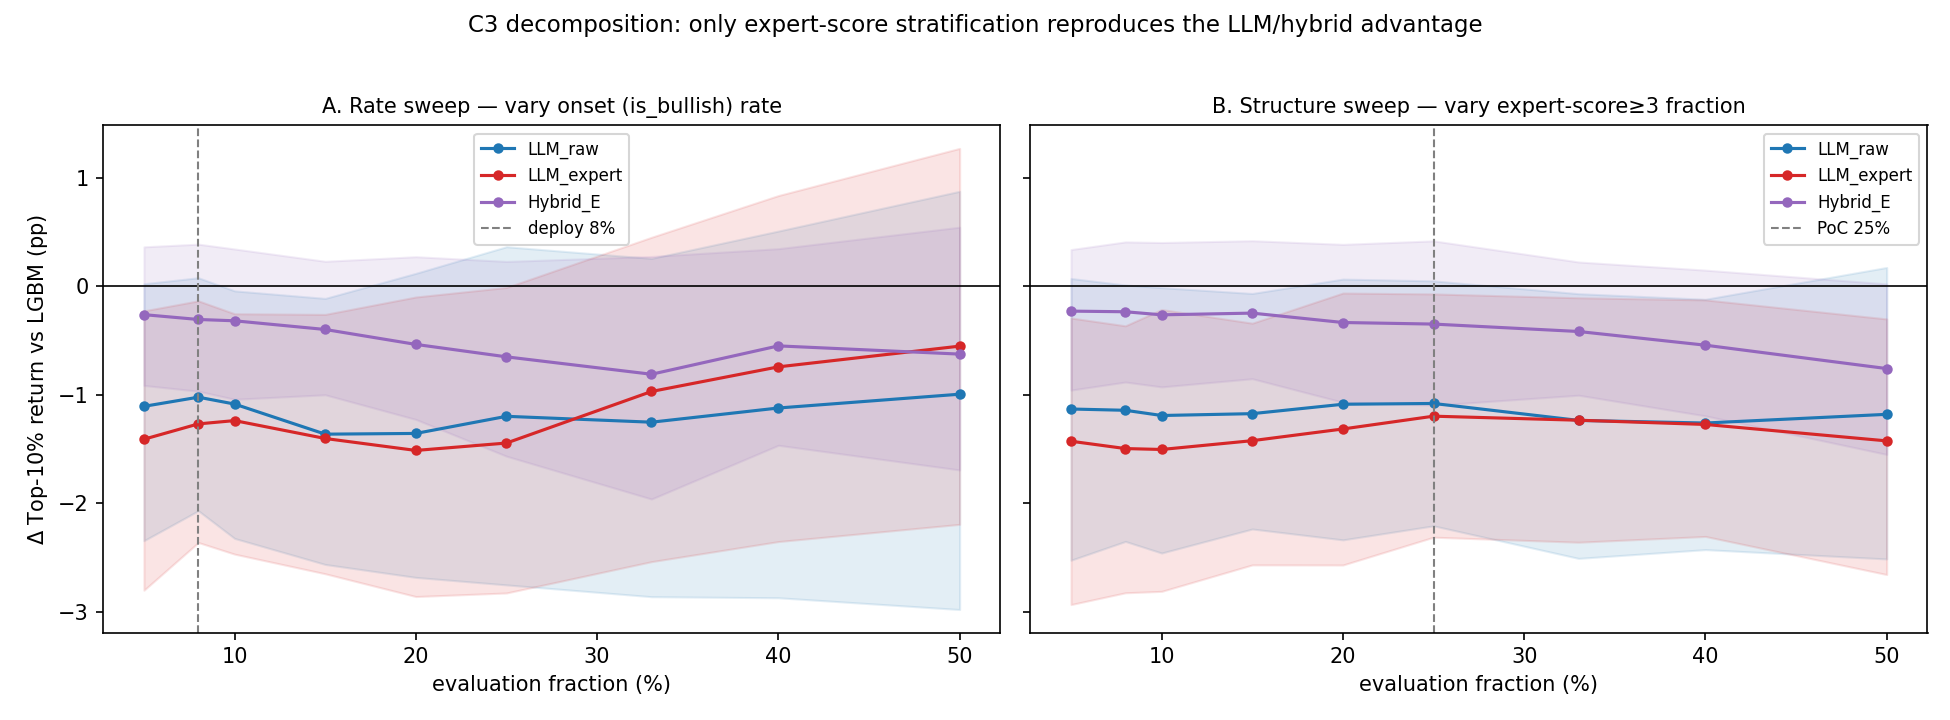
\includegraphics[width=\columnwidth]{c3_dose_response.png}
\caption{C3 dose-response: sweeping the evaluation pool's onset-rate / expert-score
composition, the hybrid's Top-10\% stays below LGBM at every composition (no
zero-crossing). Base rate is not the cause.}
\label{fig:c3}
\end{figure}

\subsection{Oracle headroom (C4) and cross-quarter heterogeneity}\label{sec:oracle}

Three different methods are optimal on the three splits (Split 1 LGBM $+3.34\%$; Split 2
LLM-raw $+1.10\%$ where LGBM fails at RankIC $-0.015$; Split 3 hybrid $+1.48\%$),
yielding a quarter-conditional oracle of $+2.02\%$ mean Top-10\% vs LGBM $+1.63\%$ ---
a $+0.39$pp upper bound for \emph{any} online router. Our four regime-aware routers
capture $\approx 0$ of it; all hybrid-vs-LGBM CIs straddle zero. Phases 2--3
(Table~\ref{tab:pattern}) instead bridge the Split-2 LGBM failure (Phase 3 RankIC
$+0.058$, Top-10\% $+1.72\%$, $+95\%$ over LGBM) at $116\times$ less labeled data and
zero deployment LLM cost.

\subsection{Temporal leakage on public benchmarks (C5 precursor)}\label{sec:leak}

We confirm (claiming no novelty) that modern LLMs leak temporally on pre-cutoff data.
On the FinBen/PIXIU stock-movement suite (Table~\ref{tab:leak},
Fig.~\ref{fig:leaksuite}), \mt{gemini-3.5-flash} scores 67--80\% directional accuracy,
but \emph{removing all input} (only ticker+date) \emph{raises} accuracy on every
benchmark, with a strong mega-cap gradient (up to 95.4\%). The identical no-context
protocol on barely-memorized A-shares falls to chance (48.6\%, CI $[45.4,51.7]$) --- a
cross-market control proving the US ``skill'' is recall, not forecasting.

\begin{table}[t]
\centering\small
\caption{Directional accuracy on the FinBen stock-movement suite. No-context $\ge$
full-context everywhere: the model predicts better with no data --- it is recalling.}
\label{tab:leak}
\begin{tabular}{lccccc}
\toprule
Benchmark & $n$ & Base & LLM ctx & \textbf{LLM no-ctx} & mega \\
\midrule
ACL18 ('14--16) & 3720 & 49.1 & 67.2 & $\mathbf{73.3}$ & 74.0 \\
BigData22 ('19--21) & 1472 & 55.2 & 60.6 & $\mathbf{71.9}$ & 73.5 \\
CIKM18 ('17) & 1143 & 53.4 & 78.8 & $\mathbf{80.3}$ & 95.4 \\
\midrule
A-share (control) & 1000 & 50.3 & --- & $\mathbf{48.6}$ & --- \\
\bottomrule
\end{tabular}
\end{table}

\begin{figure}[t]
\centering
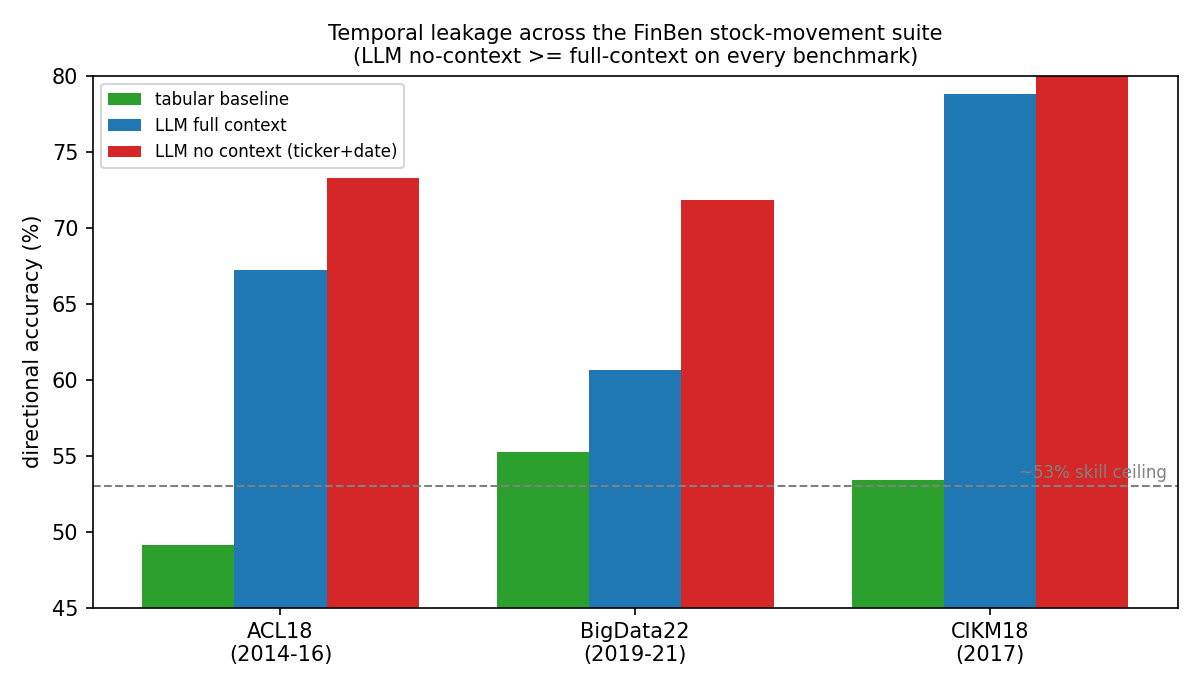
\includegraphics[width=\columnwidth]{e3_leakage_suite.png}
\caption{Temporal-leakage signature across the three FinBen benchmarks: no-context
accuracy meets or exceeds full-context, with a mega-cap gradient; the A-share control
sits at chance.}
\label{fig:leaksuite}
\end{figure}

\subsection{Leakage-free identification of the LLM's contribution (C5)}\label{sec:identify}

Leakage-freeness is an \emph{identification condition}: where the no-context probe is at
chance (A-shares), the memory channel is null, so any incremental signal is identified
as reasoning. (i) The identified LLM contribution over LGBM is $+0.033$
($[-0.037,+0.110]$) raw and $+0.006$ ($[-0.062,+0.078]$) expert --- both span zero;
the first identified (not memory-confounded) estimate, and it is $\approx 0$.
(ii) LLM-as-weak-supervisor \emph{hurts}: true-labels RankIC $+0.109$ vs LLM-refined
$-0.040$, an identified change of $-0.149$ ($[-0.298,-0.009]$). (iii) A de-biasing
estimator $\big(\text{full}-(\text{no-ctx}-\text{chance})\big)$, valid because the clean
market sits at chance, collapses FinBen to reasoning-only ACL18 0.440 / BigData22 0.388
/ CIKM18 0.485 --- at or below chance. Figure~\ref{fig:identify} summarizes.

\begin{figure}[t]
\centering
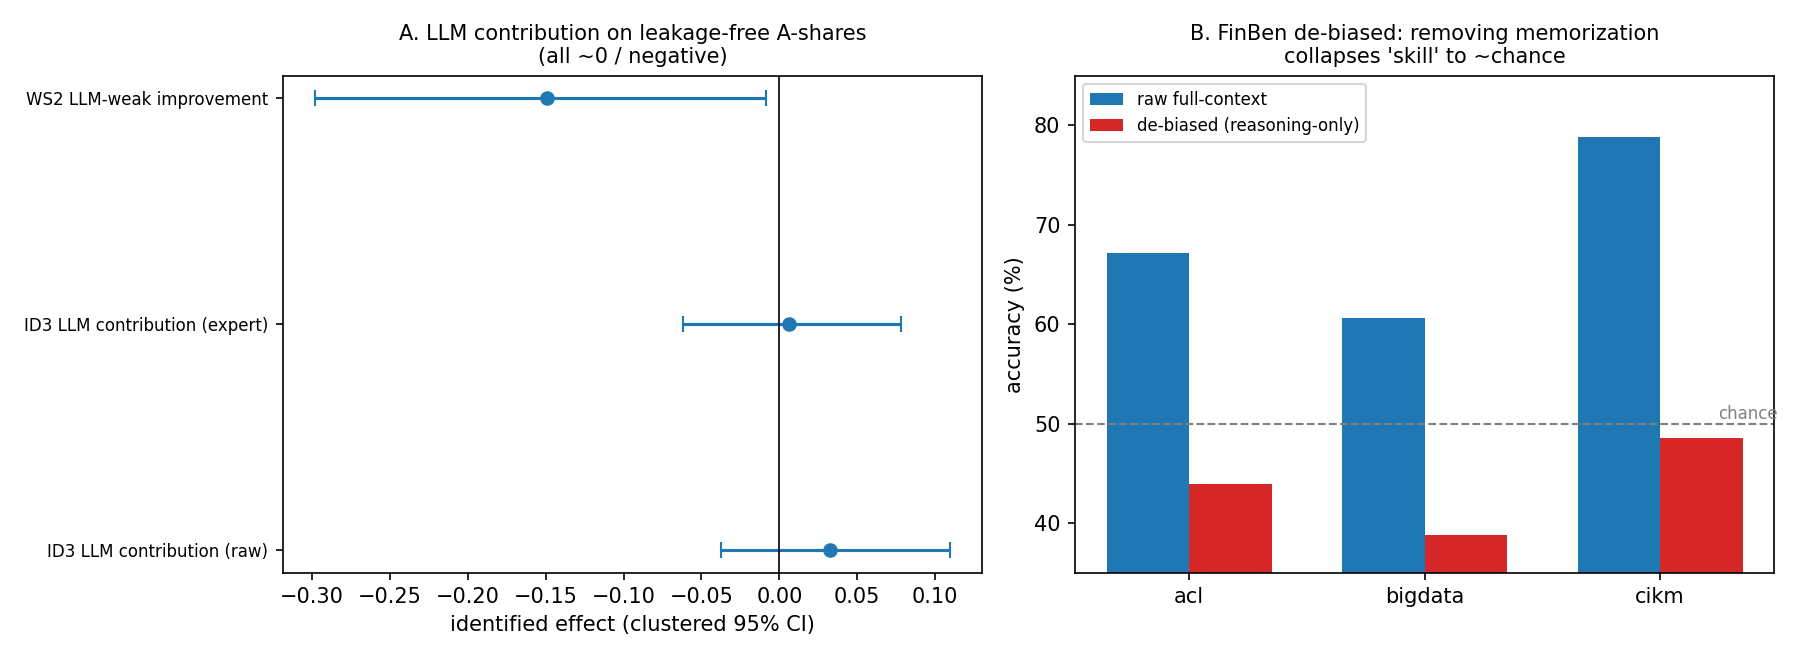
\includegraphics[width=\columnwidth]{identify_summary.png}
\caption{Leakage-free identification (C5): the identified LLM contribution to A-share
onset is $\approx 0$; weak supervision is harmful; de-biased FinBen ``skill'' collapses
to chance.}
\label{fig:identify}
\end{figure}

\subsection{Detection is not edge: the onset motif (C6)}\label{sec:motif}

The candlestick ``onset'' (relative-position geometry of recent vs prior bars) is the
strongest cross-sectional signal in the project, but a deployability gauntlet kills it:
the factors+candle long-only edge that looks good on 2025 (net Sharpe $1.10$, 3/3
splits positive) is \emph{negative} in 2023 ($-0.37$) and 2024 ($-0.36$) ---
period-specific, not deployable (Fig.~\ref{fig:deploy}). Likewise, the documented
V12.31 production rules do not reproduce the Sharpe-2.2 edge (timing is a wash,
selection is robustly negative across all knobs and OOS).

\paragraph{Is the signal merely conditional?} A natural rescue is that the onset is
informative only \emph{given} the regime (a ``promoter'' transcribed only with the right
``factor''). We test this information-theoretically. The marginal mutual information
$I(\text{pattern};r^{(5)})\approx 0$. The correct test for ``the regime adds
information'' is the interaction information $\mathrm{II}=I(X;Y\mid Z)-I(X;Y)$ with a
\emph{$Z$-label permutation} null (permuting the target within strata only tests the
trivial $I(X;Y\mid Z)>0$; at $n{=}2\times10^5$ that $p$ floors at $1/n_{\text{perm}}$).
On candlestick features $\times$ \{trend, vol, disaster\} regimes, \textbf{52/78}
feature$\times$target$\times$regime cells have $\mathrm{II}>0$; the trend regime
contributes $\approx 70$--$76\%$ of the conditional MI, and this is positive and
permutation-significant in \emph{every} year 2022--25 (Table~\ref{tab:motif},
Fig.~\ref{fig:motifmi}).

\paragraph{But MI is sign-blind.} Decomposing into conditional mean vs variance shows a
\emph{perfectly monotone} directional core (monotonicity coefficient $\approx 1.0$,
rank-slope $0.083$--$0.102$), yet only $\approx 37$--$43\%$ of the dispersion is in the
mean. The decisive test --- the simplest regime-gated long-only top-decile portfolio,
net of $\approx 0.2\%$ A-share round-trip --- yields a \emph{negative net Sharpe in
every year} despite gating improving over always-on (Fig.~\ref{fig:motiftrade}). The
gross edge ($\approx 0.1\%/$5d) sits below the cost floor. The onset motif is real,
regime-conditional, cross-period-stable, directionally monotone information --- but not
tradable alpha. The binding constraint is transaction cost, not absence of signal, sign
blindness, or non-stationarity.

\begin{table}[t]
\centering\small
\caption{Onset-motif interaction information (nats) by year, leading hits. Positive and
permutation-significant every year; absolute magnitude is small (correlation-equivalent
$\approx 0.07$--$0.14$).}
\label{tab:motif}
\begin{tabular}{llcccc}
\toprule
Feature & Regime & 2022 & 2023 & 2024 & 2025 \\
\midrule
close\_pct\_prior & trend & $+.0060$ & $+.0023$ & $+.0103$ & $+.0054$ \\
dist\_low\_atr & trend & $+.0059$ & $+.0021$ & $+.0091$ & $+.0056$ \\
onset\_score & trend & $+.0042$ & $+.0022$ & $+.0074$ & $+.0033$ \\
\bottomrule
\end{tabular}
\end{table}

\begin{figure}[t]
\centering
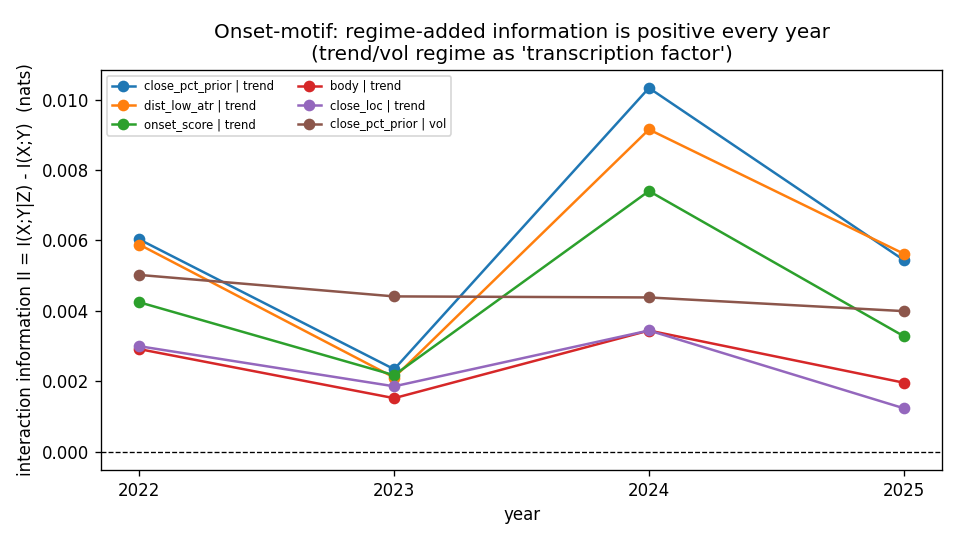
\includegraphics[width=\columnwidth]{motif_mi_summary.png}
\caption{Regime-added information (interaction information) is positive every year
2022--25 for all leading hits.}
\label{fig:motifmi}
\end{figure}

\begin{figure}[t]
\centering
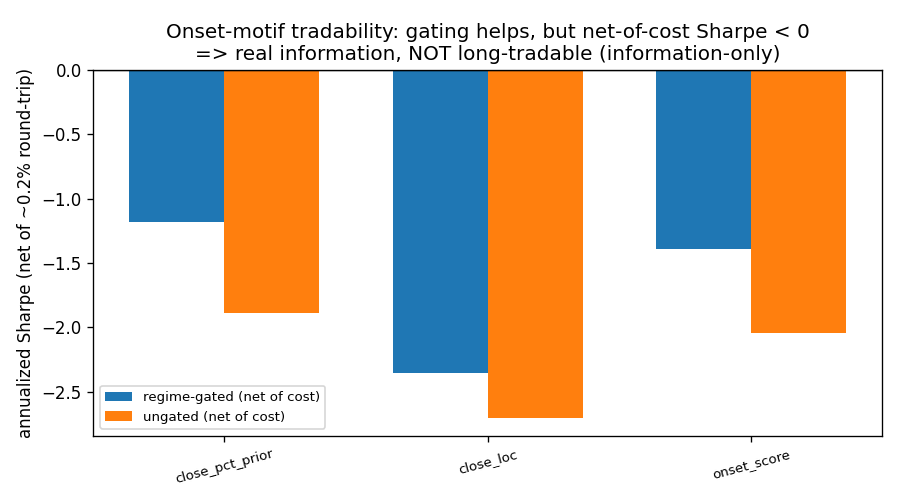
\includegraphics[width=\columnwidth]{motif_tradability.png}
\caption{Onset-motif tradability: regime gating helps, but the net-of-cost Sharpe is
negative --- real information, not long-tradable alpha.}
\label{fig:motiftrade}
\end{figure}

\begin{figure}[t]
\centering
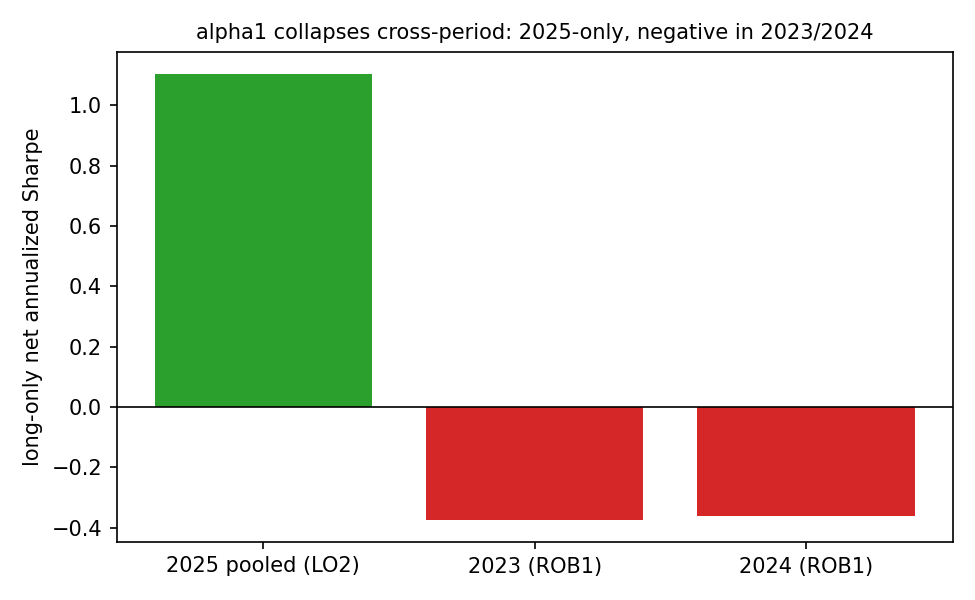
\includegraphics[width=\columnwidth]{deploy_summary.png}
\caption{Deployability gauntlet: the 2025 long-only candlestick edge collapses
cross-period (2023/2024 negative).}
\label{fig:deploy}
\end{figure}

%======================================================================
\section{Ablations and SOTA Benchmark}\label{sec:bench}

Beyond boost-magnitude, model-size (Sonnet vs Haiku), expert-prompt, sample-size, and
TCN-scaling ablations, we ask the decisive question: do recent SOTA regime/uncertainty
baselines survive our protocol? We reimplement three closest 2025--26 baselines on D1
under our exact protocol --- leakage-free walk-forward, A-share cost, non-overlapping
5-day periods, date-clustered CIs, and DSR. We do \emph{not} reproduce their US numbers
(different data/task, mostly no code); the fair test is whether their \emph{methods}
survive \emph{our} evaluation.

\begin{itemize}
\item \textbf{EXP-A --- Regime-Aware LightGBM}~\cite{regimeawarelgbm2026} (rolling-HMM
gate). One LGBM ranker, three gates. The HMM arm is the only one to clear the DSR
($0.99$), but its mean-excess CI lower bound is exactly $0.0$: its high Sharpe is a
\emph{cash-during-volatility} artifact (gating to cash shrinks the Sharpe denominator),
not selection alpha. No arm has a strictly positive net-of-cost mean CI.
\item \textbf{EXP-B --- Two-level abstention}~\cite{whenalphabreaks2026} on our onset
ranker. All arms net-negative; abstention trades 75\% of periods and stays firmly
sub-cost. It does not rescue.
\item \textbf{EXP-C --- Information-theory framings}~\cite{noguer2025fit,mukhia2026conditional}.
Marginal NMI $\le 0.0009$ --- below the $<0.05$ ``efficient-market'' band --- so NMI /
conditional-MI framings would call these features signal-free; only our interaction-info
probe isolates regime-added information (6/6 hits).
\end{itemize}

Table~\ref{tab:bench} and Figure~\ref{fig:bench} summarize: reimplemented on A-shares
under honest evaluation, the closest SOTA methods are sub-cost --- like our own signals.
Apparent regime Sharpe gains are timing/risk reduction, not net-of-cost alpha.

\begin{table}[t]
\centering\small
\caption{SOTA baselines under our protocol (pooled, net of A-share cost). DSR =
Deflated Sharpe; CI = date-clustered mean-excess. No arm has a strictly positive mean
CI.}
\label{tab:bench}
\begin{tabular}{llccc}
\toprule
Exp & Arm & Sharpe & DSR & mean CI \\
\midrule
A & plain LGBM & $+0.89$ & $0.65$ & $[-.0016,+.0036]$ \\
A & HMM-gated & $+1.92$ & $0.99$ & $[\,0.000,+.0025]$ \\
A & trend-gated & $+1.45$ & $0.82$ & $[-.0008,+.0038]$ \\
B & always-on & $-2.04$ & $0.00$ & $[-.0086,-.0031]$ \\
B & trend-gate & $-1.39$ & $0.01$ & $[-.0046,-.0008]$ \\
B & abstention & $-1.89$ & $0.00$ & $[-.0075,-.0024]$ \\
\bottomrule
\end{tabular}
\end{table}

\begin{figure}[t]
\centering
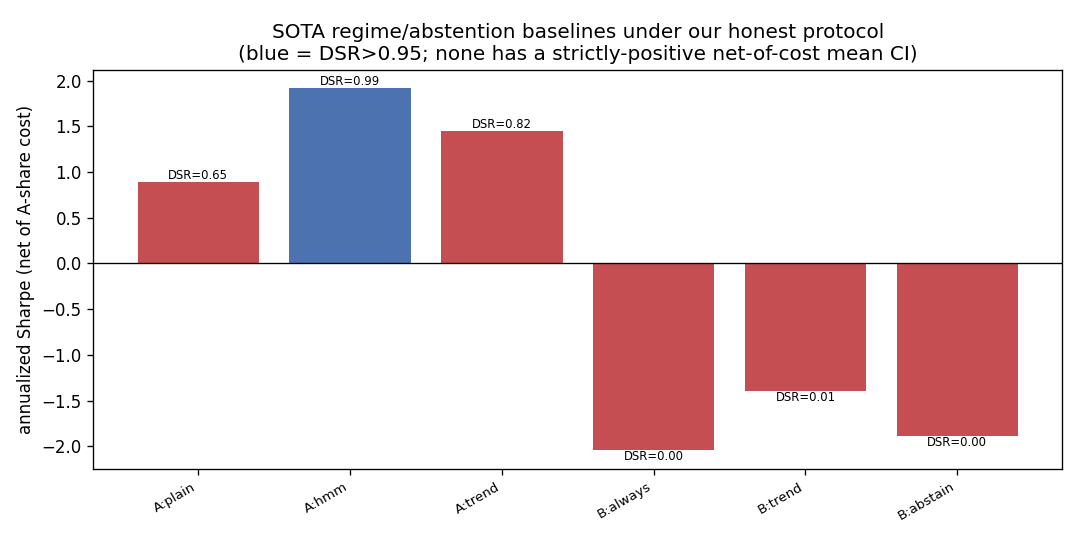
\includegraphics[width=\columnwidth]{bench_summary.png}
\caption{SOTA regime/abstention baselines under our honest protocol (blue:
DSR$>$0.95). None has a strictly positive net-of-cost mean CI.}
\label{fig:bench}
\end{figure}

%======================================================================
\section{Discussion}\label{sec:disc}

\paragraph{Why nothing trades.} Across 60+ comparisons (Fig.~\ref{fig:tree}), the only
robust positive is the onset-motif \emph{information} (C6), and it is sub-cost. The
binding constraint is transaction cost; regime conditioning buys Sharpe via
cash-during-volatility risk reduction, not alpha. This converts the thesis from ``our
signal does not trade'' into the stronger ``even 2025--26 SOTA methods, on this
substrate under honest evaluation, do not trade.''

\paragraph{Human--AI division of labor.} The two LLM architectural
limits~\cite{wang2025proactive,jiang2025hivemind} imply a clean boundary: humans supply
the edge hypothesis (``who pays you, and why?''); the AI's value is rigorous execution
and adversarial falsification (estimators, cost models, permutation nulls, walk-forward,
DSR). Our onset-motif probe arose exactly this way --- a human analogy plus an
AI-built information-theoretic test --- not from asking an LLM to ``find alpha.''

\paragraph{Limitations.} Single market (A-shares); three quarterly test splits
(mitigated by date-clustered CIs); a single LLM family for the agent experiments;
public features only --- we make no claim about proprietary microstructure data.

%======================================================================
\section{Conclusion}\label{sec:concl}

We presented V12-Agentic and a leakage-free, cost-aware audit of LLM and regime methods
for A-share movement-onset detection. The identified LLM contribution is $\approx 0$;
candlestick onset information is real, regime-conditional, and cross-period-stable yet
sub-cost; and reimplemented SOTA baselines are also sub-cost under our protocol. The
contributions are the honest evaluation machinery (date-clustered CIs, realistic costs,
cross-period gates, Deflated Sharpe, interaction-information probing) and a precise
localization of why \emph{detection is not edge}. We release the harness, the
walk-forward sampler, the information-theoretic probes, and the V12.31 expert prompt.

\bibliographystyle{ACM-Reference-Format}
\bibliography{references}

\appendix
\section{V12.31 Expert Prompt}
The full $\sim$5{,}500-character elicited expert prompt (bullish-onset rules
$C1$--$C4$, bearish asymmetry, disaster composite) is provided in
\mt{prompts/v12\_31\_expert\_v1.md} and reproduced in the supplementary material.

\end{document}
